\documentclass[10pt,a4]{article}

%\usepackage[toc,page]{appendix}
\usepackage{geometry}
\usepackage{amsmath}
\usepackage{physics}
\usepackage{graphicx}
\usepackage{mathtools}      % loads amsmath and some very useful complements
\usepackage{booktabs}       % professional-quality tables
\usepackage{amsfonts}       % blackboard math symbols
\usepackage{nicefrac}       % compact symbols for 1/2, etc.
\usepackage{microtype}      % microtypography
\usepackage{textcomp}       % registered and trademark symbols

\usepackage[colorlinks,linkcolor=black,citecolor=blue,urlcolor=blue]{hyperref}

\usepackage[ruled,vlined]{algorithm2e}  % used for including algorithms
\usepackage{subcaption}                 % needed for using subfigures
\usepackage{amssymb}
\usepackage{physics}
\usepackage{verbatim} 
\usepackage{fancyhdr}
\usepackage{hyperref}
\usepackage{cleveref}   % must come after hyperref, see https://ctan.org/pkg/cleveref and https://www-uxsup.csx.cam.ac.uk/pub/tex-archive/macros/latex/contrib/cleveref/cleveref.pdf

% code listings
% -------------
\usepackage{color}
\definecolor{dkgreen}{rgb}{0,0.6,0}
\definecolor{gray}{rgb}{0.5,0.5,0.5}
\definecolor{mauve}{rgb}{0.58,0,0.82}

\usepackage{listings}
\lstset{frame=tb,
  language=Python,
  aboveskip=3mm,
  belowskip=3mm,
  showstringspaces=false,
  columns=flexible,
  basicstyle={\small\ttfamily},
  numbers=none,
  numberstyle=\tiny\color{gray},
  keywordstyle=\color{blue},
  commentstyle=\color{dkgreen},
  stringstyle=\color{mauve},
  breaklines=true,
  breakatwhitespace=true,
  tabsize=3,
  captionpos=b
}

\lstdefinelanguage{json}{
  sensitive = true,
  basicstyle={\small\ttfamily},
  numberstyle=\tiny\color{gray},
  keywordstyle=\color{blue},
  stringstyle=\color{mauve},
  morestring=[b]',
  morestring=[b]"
}

\lstdefinelanguage{console}{
}

%
% add listings to cleveref
% ------------------------
\crefname{lstlisting}{listing}{listings}
\Crefname{lstlisting}{Listing}{Listings}

%
% nomenclature
% ------------
\usepackage{nomencl}
\makenomenclature
\renewcommand{\nomname}{Notation}

%
% path for figures
% ----------------
\graphicspath{{figures/}}

% page layout
% -----------
\geometry{verbose,a4paper,tmargin=25mm,bmargin=25mm,lmargin=25mm,rmargin=25mm}

%
% header
% ------
\pagestyle{fancy}
\renewcommand{\headrulewidth}{0.5pt} % line in header area
\fancyhf{}
\chead{1D Nozzle Solver for QLES}
\cfoot{\thepage}


% Front page
% ----------
\title{A Python Framework for Solving 1-Dimensional Nozzle Flows using Quantum Linear Equation Solvers}
\author{
  Leigh Lapworth \\
  Rolls-Royce
}

\begin{document}
\maketitle

% abstract
% --------
\begin{abstract}
This article describes a hybrid quantum-classical testing framework for the 1-dimensional
flow through a convergent-divergent nozzle.
The CFD solver models both low-speed incompressible and transonic compressible flow.
It also offers both the segregated SIMPLE solver and an implicit coupled solver for both 
flow types.
The core solver is written in C and is accessible via a Python wrapper using the {\it ctypes}
interface.
This allows the solver to be tested with a range of quantum computing APIs.
The solver is controlled using a simple XML file.
The Python interface using a simple get and put interface to retrieve the CFD matrix and
right hand side vector from the CFD discretisation and return the QLES solution to update the 
flow field.
There are a range of solver options that can be used to generate matrices with up to 8 diagonals 
using the coupled compressible solver. The standard pressure correction solver has 3 diagonals.
The coupled incompressible solver has 6 diagonals and gives rapid convergence which is useful when
emulating the quantum circuit is time-consuming.
\end{abstract}


% Nomenclature
% ------------
\printnomenclature

% Contents
% --------
\newpage
\tableofcontents

% sections  (\input preferred as \include adds a clear page)
% --------
\newpage
% Nomenclature file
% 
% To refresh type: make
%                  make nomen
%                  make
%
% See https://texblog.org/2012/05/14/list-of-symbols-or-abbreviations-nomenclature/

\nomenclature{$c_p$}{specific heat capacity at constant pressure, $c_p = \frac{\gamma}{\gamma-1} R$}
\nomenclature{$c_v$}{specific heat capacity at constant volume}
\nomenclature{$\gamma$}{ratio of specific heats, $\gamma = \frac{c_p}{c_v}$}
\nomenclature{$M$}{Mach number = velocity/speed of sound, $M = \frac{u}{\sqrt{\gamma R t}}$}
\nomenclature{$p$}{static pressure}
\nomenclature{$P_0$}{stagnation pressure}
\nomenclature{$R$}{perfect gas constant, $R = c_p - c_v$}
\nomenclature{$t$}{static temperature}
\nomenclature{$T_0$}{stagnation temperature}
\nomenclature{$u$}{axial velocity}


%
% Introduction
% ------------
\section{Introduction}

The 1D nozzle solver provides a flexible Python interface for testing quantum linear equation
solvers on fluid flow type problems.
The core CFD solver, written in C, is linked via a library to enable developers to focus on their
quantum solver.

The benefit of the nozzle system is that it allows researchers to investigate the feedback between the
inner linear system, solved using a quantum algorithm, and the outer classical non-linear update.
\cite{lapworth2022implicit} has shown the performance of HHL \cite{harrow2009quantum}, relative to a classical linear
solver, must be assessed within the context of the convergence of the non-linear CFD solver.
For HHL, there is a specific iterative feed-forward mechanism associated with the 
under-resolution of the eigenvalue spectrum.
Similar behaviour is anticipated with other linear solvers such as 
Quantum Singular Value Transformation (QSVT)
\cite{martyn2021grand, gilyen2019quantum, dong2021efficient}
, albeit as a result of different mechanisms.

Although the solver is only 1 dimensional, there are a range of solver options that can be
used to generate matrices with up to 8 diagonals using the coupled compressible solver. The standard
pressure correction solver has 3 diagonals. The coupled incompressible solver has 6 diagonals and
gives rapid convergence which is useful when emulating the quantum circuit is time-consuming.

The plotting routines enable easy comparison of classical and quantum results.




%
% Solver
% ------------
\section{Nozzle CFD}

Throughout this document the test case is referred to as a {\it nozzle}.
This is the more common terminology for transonic flows. 
For incompressible flows, {\it channel} is more commonly used, but we use a
single terminology for both flow regimes.

\begin{figure}[ht]
  \begin{center}
    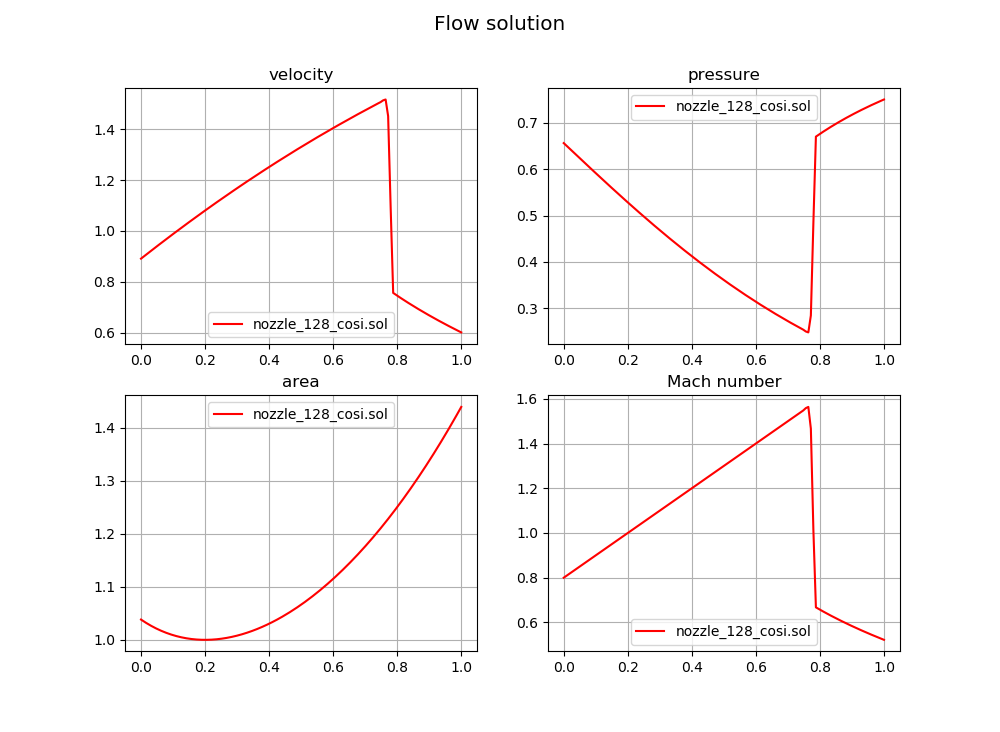
\includegraphics[width=0.70\textwidth]{c128-sol-simple.png}
  \end{center}
  \caption{Solution for compressible nozzle with 128 stations.}
  \label{fig-c128-sol-simple}
\end{figure}

\Cref{fig-c128-sol-simple} shows the converged flow solution for a transonic 
compressible test case.
The bottom left figure shows the area of the channel, $A$, which is derived from the
isentropic flow relationships:

\begin{equation}
  \frac{A}{A^*} = \frac{1}{M}
                  \left[ \frac{2}{\gamma+1} \left(1 + \frac{\gamma - 1}{2}M^2 \right)
                  \right]^{\frac{\gamma+1}{2(\gamma - 1)}}
  \label{eqn:isent-area}
\end{equation}

where $M$ is the Mach number, $\gamma$ is the ratio of specific heats and
$A^*$ is the area at the throat where $M=1$.
In this test case, all variables are non-dimensionalised so that $A^*=1$.
The length of the nozzle is always set to 1 and the user specifies an inlet Mach number, $M_{in}$.
To set-up the nozzle area distribution, the outlet Mach number is set to $M_{out} = 1+M_{in}$.
The axial stations are set according an equal Mach number of increment of
$\delta M = 1.0/(nx-1)$ where $nx$ is the number of axial stations in the mesh. 
The area at each station is set from \Cref{eqn:isent-area}.
Note that the area equation is for isentropic, i.e. reversible, flow where the Mach number
increases linearly. In the absence of a shock wave this gives the CFD solution.
However, the interest is in the case when there is a shock wave within the nozzle as shown 
in the bottom right of \Cref{fig-c128-sol-simple}.

For incompressible flows, the channel area is an arc of a circle with a specified
area contraction, typically $10\%$ at the midpoint, relative to the inlet and exit areas
which are both set to $1.0$. The area distribution is not shown but follows the shape
of the pressure distribution.

\begin{figure}[ht]
  \begin{center}
    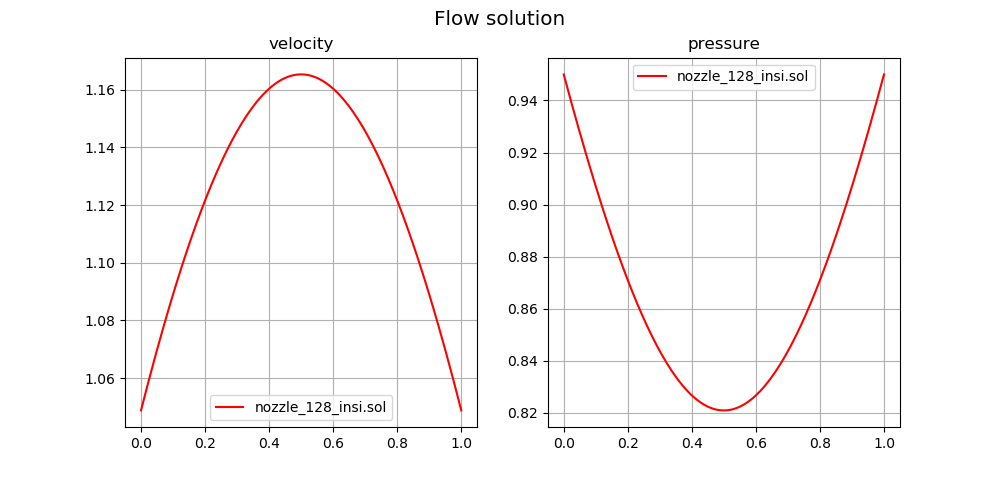
\includegraphics[width=0.70\textwidth]{i128-sol-simple.png}
  \end{center}
  \caption{Solution for incompressible nozzle with 128 stations.}
  \label{fig-i128-sol-simple}
\end{figure}


%
% Boundary conditions
% -------------------
\subsection{Boundary Conditions}

In addition to setting the geometry of the nozzle, we also need to provide boundary
conditions at the entrance and exit to the nozzle. These must be specified in a way that
is consistent with that signals propogate within the flow.

Following \Cref{fig-nozzle-disc}, a velocity boundary condition is set at the inlet as
the velocity updates are largely convected in the flow direction.
a pressure boundary condition is set at the outlet, as pressure signals propogate in 
all directions at the speed of sound, relative to the flow field. 
Setting an exit pressure boundary condition is only physically valid when the exit 
flow velocity is subsonic. This is case for both incompressible and compressible flows
used here and, hence, both have the same form of outlet condition:

\begin{equation}
  p|_{i=n}  = p_{exit}
  \label{eqn-inletbc}
\end{equation}

That is, $p$ at the exit station, $i=n$ has a fixed value, $p_{exit}$.
Although, incompressible and compressible flows have the same form of exit boundary
condition, the values are different.
The compressible solution in \Cref{fig-c128-sol-simple} has $p_{exit} = 0.75$.
Whereas, the incompressible solution in \Cref{fig-i128-sol-simple} 
has $p_{exit} = 0.95$.

For both compressible and incompressible flows, the values of velocity at the exit and
the pressure at the inlet are computed from the solution of the flow equations.
At the inlet, the computed inlet value of pressure is used to set an inlet velocity 
according to the inflow boundary condition. 

\subsubsection{Compressible inflow condition}

For compressible flows, the isentropic relationships give:

\begin{equation}
  \left( \frac{T_0}{t} \right ) =  \left( \frac{P_0}{p} \right ) ^{\frac{\gamma-1}{\gamma}}
  \label{eqn-t-p-isen-1}
\end{equation}

Where $T_0$ and $P_0$ are the staganation temperature and pressure which are constant in
isentropic, i.e. shock-free, flows.
The flow upstream of the nozzle inlet is taken as isentropic and $T_0$ and $P_0$ 
are user-specified boundary values. 
For non-dimensionalised conditions, as used here, it is usual to set them both to unity.

Rearranging \Cref{eqn-t-p-isen-1} gives:
\begin{equation}
  t = T_0 \left( \frac{p}{P_0} \right ) ^{\frac{\gamma-1}{\gamma}}
  \label{eqn-t-p-isen-2}
\end{equation}

In addition, we have conservation of energy which, for isentropic flow, can be 
expressed in terms of temperature as:

\begin{equation}
  T_0 = t + \frac{1}{2c_p}u^2
  \label{eqn-energy}
\end{equation}

And can be rearranged to give:

\begin{equation}
  u = \sqrt{2 c_p (T_0 - t)}
  \label{eqn-uin-isen}
\end{equation}

\Cref{eqn-t-p-isen-2} and \Cref{eqn-uin-isen} allow the inlet velocity to be updated from
the value of pressure and the specified inlet stagnation conditions.


\subsubsection{Incompressible inflow condition}

For incompressible flow, we cannot use the isentropic relations as strictly the Mach number is
zero or, more accurately, the speed of sound is infinite. Instead, we uswe Bernoulli's equation:

\begin{equation}
  P_0 = p + \frac{1}{2}\rho u^2
  \label{eqn-Bernoulli}
\end{equation}

From which, the inlet velocity can be set from the computed inlet static pressure and
the specified inlet stagnation pressure:

\begin{equation}
  u = \sqrt{\frac{2}{\rho} (P_0 - p)}
  \label{eqn-uin-bern}
\end{equation}



% Discretisation
% --------------
\subsection{CFD discretisation}
\label{subsec-discrete}

Since, the focus of this test case is not CFD development, we use the discretisation scheme of
\cite{gupta1993development}. In this scheme, the velocities and pressures are stored at the 
same set of nodes with upwinded momentum control volumes and downwinded continuity control
volumes. These are show in \Cref{fig-nozzle-v-disc} and \Cref{fig-nozzle-disc} respectively.

\begin{figure}[h]
  \centering
  \begin{subfigure}[b]{0.70\textwidth}
      \centering
      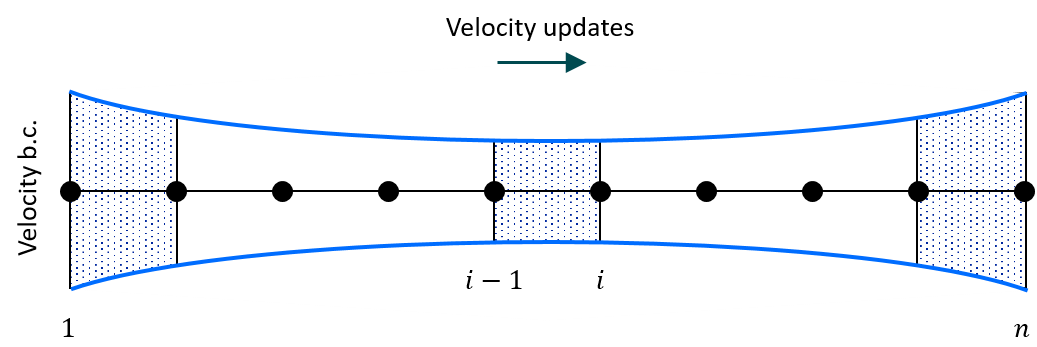
\includegraphics[width=\textwidth]{nozzle-v-disc.png}
      \caption{Upwinded momentum control volumes used to update nodes 2,..,n.}
      \label{fig-nozzle-v-disc}
  \end{subfigure}
  \hfill
  \begin{subfigure}[b]{0.70\textwidth}
      \centering
      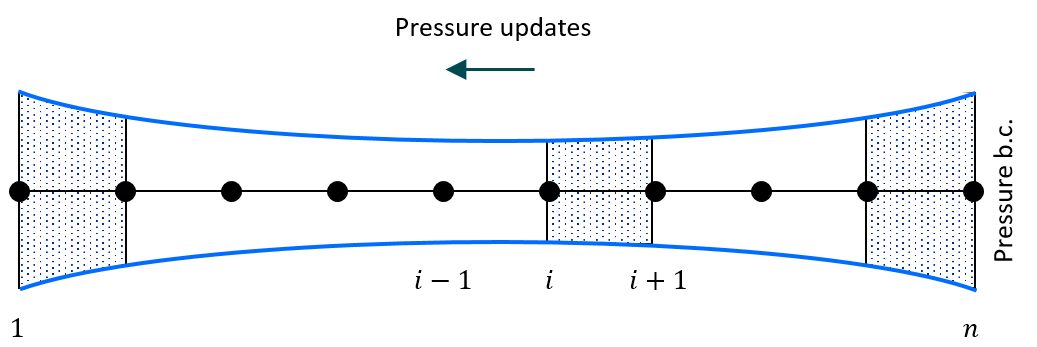
\includegraphics[width=\textwidth]{nozzle-p-disc.png}
      \caption{Downwinded continuity control volumes used to update nodes 1,..,n-1.}
      \label{fig-nozzle-p-disc}
  \end{subfigure}
  \caption{Control volume setting for momentum and continuity equations.}
  \label{fig-nozzle-disc}
\end{figure}

The 1-dimensional steady state equations to be solved are:

\begin{equation}
  \begin{array}{rcl}
    \rho u \frac{\partial u}{\partial x} &=& - \frac{\partial p}{\partial x} \\[8pt]
    \frac{\partial \rho u}{\partial x} &=& 0 \\
  \end{array}
  \label{eqn-euler-1d}
\end{equation}

For compressible flows, the following equations are also applied:

\begin{equation}
  \begin{array}{rcl}
    p   &=& R\rho t \\[8pt]
    T_0 &=& t + \frac{1}{2c_p}u^2
  \end{array}
  \label{eqn-gaslaw}
\end{equation}

where $R$ is the gas constant, $c_p$ is the specific heat at constant pressure, and
$T_0$ is the constant total temperature which is set in $1.0$ in non-dimensional 
units. This equation represents the conservation of energy. 


The differential equations are discretised on the 1-dimensional mesh and 
updated iteratively via corrections:
\begin{equation}
  \begin{array}{rcl}
     \ket{u}    &\gets& \ket{u}    + \ket{\delta u} \\[8pt]
     \ket{p}    &\gets& \ket{p}    + \ket{\delta p} \\[8pt]
     \ket{\rho} &\gets& \ket{\rho} + \ket{\delta \rho}
  \end{array}
  \label{eqn-iter-update}
\end{equation}

For incompressible cases, the density is fixed at a non-dimensional value of $1.0$ 
and is not updated as part of the solution. 

The coupled iterative scheme is the most conceptually straightforward and will
be described first


% Incompressible Coupled
% ----------------------
\subsubsection{Incompressible coupled solver}
\label{subsubsec-inco-couple}

For incompressible flow, the discrete version of momentum equation is \Cref{eqn-euler-1d} is:

\begin{equation}
  \begin{array}{rcl}
    \rho u_{i-\frac{1}{2}} \frac{u_i - u_{i-1}}{x_i - x_{i-1}} &=&
                   - \frac{p_i - p_{i-1}}{x_i - x_{i-1}} \\
  \end{array}
  \label{eqn-euler-1d-disc1}
\end{equation}

Note that we have followed \cite{gupta1993development} in using a finite difference
discretisation for the momentum equation.


It is common practice in CFD to form an {\it inner} linearised system
to solve for the corrections. The only non-linear term in \Cref{eqn-euler-1d-disc1} is
the term on the left hand side of the first equation. 
Following \cite{gupta1993development},
this is linearised using a fixed point iterative scheme for the momentum equation to give:

\begin{equation}
  \begin{array}{rcl}
    \rho u_{i-\frac{1}{2}} (u_i + \delta u_i - u_{i-1} - \delta u_{i-1}) &=&
                   - (p_i + \delta p_i - p_{i-1} - \delta p_{i-1} ) \\[8pt]
    \rho u_{i-\frac{1}{2}} (\delta u_i - \delta u_{i-1}) +
    (\delta p_i - \delta p_{i-1}) &=&
    -\rho u_{i-\frac{1}{2}} (u_i - u_{i-1}) -
    (p_i - p_{i-1}) \\[8pt]
    &=& R_i^u
  \end{array}
  \label{eqn-euler-1d-disc2}
\end{equation}

We have also followed \cite{gupta1993development} in using a finite difference
discretisation for the momentum equation.

For the continuity equation, we use a finite volume discretisation to give
\begin{equation}
  \begin{array}{rcl}
    A_{i+1}\rho u_{i+1} - A_{i}\rho u_{i} &=& 0 \\[8pt]
    A_{i+1}\rho \delta u_{i+1} - A_{i}\rho \delta u_{i} &=&
    -(A_{i+1}\rho u_{i+1} - A_{i}\rho u_{i}) \\[8pt]
    &=& R_i^p
  \end{array}
  \label{eqn-euler-1d-disc3}
\end{equation}

Where $R_u^i$ and $R_p^i$ are the errors in satisfying the flow equations at node $i$,
these are usually called the residuals.

We must also linearise the incompressible inlet boundary condition from \Cref{eqn-Bernoulli}:

\begin{equation}
  \begin{array}{rcl}
    p_1 + \delta p_1 + \frac{1}{2} \rho (u_1 + \delta u_1) ^2 &=& P_0 \\[8pt]
          \delta p_1 + \rho u_1 \delta u _1&=& P_0 - p_1 - \frac{1}{2} \rho u_1^2 \\[8pt]
          \delta p_1 + \rho u_1 \delta u_1 &=& R^u_1
  \end{array}
  \label{eqn-incomp-in-disc1}
\end{equation}

The exit boundary condition is simply:
\begin{equation}
  \delta p_n = p_{exit} - p_n
  \label{eqn-incomp-ex-disc1}
\end{equation}


Collecting together the discrete momentum and continuity equations leads to a set of
simultaneous equations that can be expressed in block matrix form as:


\begin{equation}
  \begin{pmatrix}
    A^u + B^{u_1} & D^x + B^{p_1} \\
    M^x           & B^{p_n} \\
  \end{pmatrix}
  \begin{pmatrix}
    \ket{\delta u} \\
    \ket{\delta p}
  \end{pmatrix}
  = 
  \begin{pmatrix}
    \ket{R^u} \\
    \ket{R^p}
  \end{pmatrix}
  \label{eqn-implicit-01}
\end{equation}

Where
\begin{itemize}
    \item $A^u$ is the matrix containing the discrete convection operator 
                for the $u$ momentum equation.
    \item $B^{u_1}$ and $B^{p_1}$ are the the entries for the discretied inlet velocity boundary condition.
    \item $D^x$ is the discrete pressure gradient operator.
    \item $M^x$ is the the discrete continuity operator.
    \item $B^{p_n}$ is the the entry for the discretised outlet pressure boundary condition.
    \item $R^u$ and $R^p$ are the residuals of the momentum and continuity equations.
\end{itemize}

\Cref{fig-i16-cpl-sparse} shows the sparsity pattern for an implicit coupled incompressible
matrix with 16 mesh nodes.
Row 0 corresponds to the inlet boundary condition.
Rows 1-15 are the momentum equations up to the exit node.
Rows 16-30 are the continuity equations starting at the inlet node.
Row 31 is the exit boundary condition.

\begin{figure}[h]
  \begin{center}
    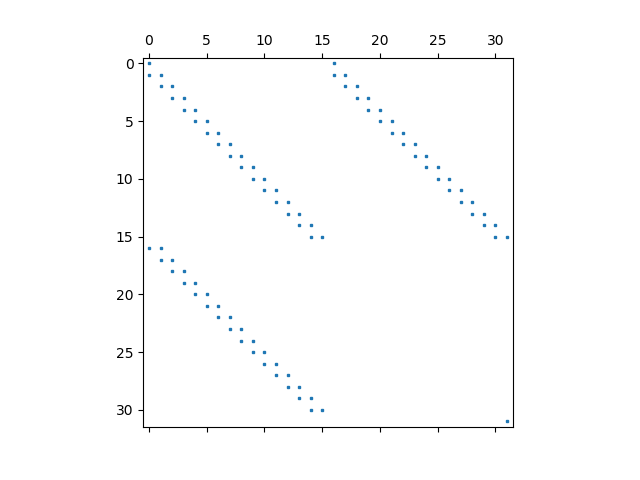
\includegraphics[width=0.60\textwidth]{i16_cpl_sparse.png}
  \end{center}
  \caption{Incompressible nozzle with 16 stations, sparsity pattern for coupled matrix.}
  \label{fig-i16-cpl-sparse}
\end{figure}


\Cref{tab-imp-incomp} provides details for a range of mesh sizes for
incompressible implicit matrices. The dimensions of the Hermitian matrix are do the symmetrised
matrix needed by HHL. The number of unitaries are derived from the decomposition of
the Hermitian matrix into Pauli strings.
The number of CFD iterations are those required to reduce the residuals and 
corrections to less than $1 \times 10^{-12}$.

\begin{table}[h]
  \centering
  \begin{tabular}{c c c c c c c}
    \toprule
    Nstations & Hermitian matrix &  $\lambda_{min}$ & $\lambda_{max}$ & $\kappa$ & Nunitaries & CFD iterations \\
    \midrule
     8   &   32x32     &$7.9\times10^{-2}$ & 3.32      & 42.1     & 128   &  5  \\
     16  &   64x64     &$3.9\times10^{-2}$ & 3.36      & 86.1     & 316   &  5  \\
     32  &  128x128    &$1.9\times10^{-2}$ & 3.38      & 173      & 740   &  5  \\
     64  &  256x256    &$9.6\times10^{-3}$ & 3.39      & 348      & 1,752 &  5  \\
    \bottomrule
  \end{tabular}
  \caption{Incompressible implicit matrices.
           Dimensions, eigenvalue range, condition number and number of unitaries in LCU.
           Sampled after at end of run. Area contraction = 10\%.}
  \label{tab-imp-incomp}
\end{table}



% Compressible Coupled
% --------------------
\subsubsection{Compressible coupled solver}
\label{subsubsec-comp-couple}

For compressible flows, the implicit discretisation combines the gas law and energy equations
to give:

\begin{equation}
  \begin{array}{rcl}
    p_i + \delta p_i &=& R (\rho_i + \delta \rho_i)(T_0 - \frac{1}{2c_p}(u_i + \delta u_i)^2) \\[8pt]
                     &=& R\rho_i(T_0 - \frac{1}{2c_p}(u_i^2 + 2 u_i \delta u_i)) +
                         R \delta \rho_i (T_0 - \frac{1}{2c_p}u_i^2) \\[8pt]
                     &=& R\rho_i t_i + \frac{R}{c_p} \rho_i u_i \delta u_i + Rt_i \delta \rho_i 
  \end{array}
  \label{eqn-euler-1d-disc4}
\end{equation}

Collecting the terms together gives:
\begin{equation}
  \begin{array}{rcl}
   -\frac{R}{c_p} \rho_i u_i \delta u_i + \delta p_i - Rt_i \delta \rho_i &=& R\rho_i t_i - \delta p_i \\[8pt]
      &=& R_{\rho}^i
  \end{array}
  \label{eqn-euler-1d-disc5}
\end{equation}

There is one further aspect to the implementation of the gas law which is due to the fact
that the continuity control volumes are {\it downwinded} as shown in \Cref{fig-nozzle-p-disc}.
To maintain stability at supersonic Mach numbers the perfect gas must compensate for this by
using an upwinded effective pressure:

\begin{equation}
    \rho = \frac{1}{Rt} p_{eff}
  \label{eqn-peff1}
\end{equation}

For Mach numbers less than 2, this is discretised as \cite{gupta1993development}:

\begin{equation}
   p_{eff,i} = p_{i-1} + a_0(p_i - p_{i-1}) + \frac{a_1}{2} (p_i - p_{i-2})
  \label{eqn-peff2}
\end{equation}

Where
\begin{equation}
  \begin{array}{rcl}
    a_0 &=& \frac{0.8}{3} (\frac{4}{M^2} - 1) \\[8pt]
    a_1 &=& 1.0 - a_0
  \end{array}
  \label{eqn-peff3}
\end{equation}

Where $M$ is the local maximum Mach number between stations $i$ and $i-1$.
For low subsonic flow, $a_0=1$ and $a_1 = 01$ giving $p_{eff,i} = p_i$, i.e. no upwinding.

For the implicit discretisation, only the first order upwinding correction is retained.
Hence, \Cref{eqn-euler-1d-disc5} becomes:

\begin{equation}
   -\frac{R}{c_p} \rho_i u_i \delta u_i + \delta p_i - Rt_i \delta \rho_i = 
    R\rho_i t_i - \delta p_{i-1} - a_0(\delta p_i - \delta p_{i-1}) \\
  \label{eqn-euler-1d-disc6}
\end{equation}

We must also linearise the compressible inlet boundary condition from \Cref{eqn-energy}:

\begin{equation}
  \begin{array}{rcl}
    t_1 + \delta t_1 + \frac{1}{2c_p} (u_1 + \delta u_1) ^2 &=& T_0 \\[8pt]
    t_1 + \delta t_1 + \frac{1}{c_p} u_1 \delta u_1 &=& T_0 - \frac{1}{2c_p} \rho u_1^2 \\[8pt]
    t_1 + \delta t_1 + \frac{1}{c_p} u_1 \delta u_1 &=& R^u_1
  \end{array}
  \label{eqn-comp-in-disc1}
\end{equation}

Linearising \Cref{eqn-t-p-isen-2} gives:
\begin{equation}
  \begin{array}{rcl}
    t_1 + \delta t_1 &=& T_0 \left( \frac{p_1}{P_0} \right ) ^{\frac{\gamma-1}{\gamma}}
                             \left(1 + \frac{\delta p_1}{p_1} \right ) ^{\frac{\gamma-1}{\gamma}} \\[8pt]
                     &=& T_0 \left( \frac{p_1}{P_0} \right ) ^{\frac{\gamma-1}{\gamma}}
                             \left(1 + \frac{\gamma-1}{\gamma}\frac{\delta p_1}{p_1} \right )
  \end{array}
  \label{eqn-t-p-isen-3}
\end{equation}

Combining \Cref{eqn-comp-in-disc1} and \Cref{eqn-t-p-isen-3} gives:
\begin{equation}
  \begin{array}{rcl}
     \frac{1}{c_p} u_1 \delta u_1 + 
     \frac{T_0}{p_1} \left( \frac{p_1}{P_0} \right ) ^{\frac{\gamma-1}{\gamma}} \frac{\gamma-1}{\gamma}\delta p_1  &=&
     T_0 -T_0 \left( \frac{p_1}{P_0} \right ) ^{\frac{\gamma-1}{\gamma}} - \frac{1}{2c_p} \rho u_1^2 \\[8pt]
     \frac{1}{c_p} u_1 \delta u_1 +
     \frac{T_0}{p_1} \left( \frac{p_1}{P_0} \right ) ^{\frac{\gamma-1}{\gamma}} \frac{\gamma-1}{\gamma}\delta p_1 &=& R^u_1
  \end{array}
  \label{eqn-comp-in-disc2}
\end{equation}

The exit boundary condition is the same as \Cref{eqn-incomp-ex-disc1}.


The fixed point iteration means that the compressible discretisation is the same as the 
compressible one except that the local density is used rather than the constant one.
The compressible continuity equation is straightforward application of corrections to the
velocity and density. This leads to a coupled compressible matrix of the form:

\begin{equation}
  \begin{pmatrix}
    A^u + B^{u_1} & D^x + B^{p_1} & 0        & 0 \\
    M^u           & B^{p_n}       & M^{\rho} & 0 \\
    L^u           & L^p           & L^{\rho} & 0 \\
    0             & 0             & 0        & I \\
  \end{pmatrix}
  \begin{pmatrix}
    \ket{\delta u}    \\
    \ket{\delta p}    \\
    \ket{\delta \rho} \\
    \ket{\psi}        \\
  \end{pmatrix}
  = 
  \begin{pmatrix}
    \ket{R^u} \\
    \ket{R^p} \\
    \ket{R^{\rho}} \\
    \ket{0} \\
  \end{pmatrix}
  \label{eqn-implicit-02}
\end{equation}

where the newly introduced terms are:
\begin{itemize}
    \item $L^u$, $L^p$ and $L^\rho$ are the coefficients from the gas law discretisation.
    \item $M^{\rho}$ are the additional terms from the dicretisation of $\rho$ in the 
                continuity equation.
    \item $I$ is a diagonal block that is required to extend the matrix so that it has a 
              full rank equal to a power of 2. $\ket{\psi}$ are the corresponding entries in
              the state vector and the matrix solution ensures $\ket{\psi} = \ket{0}$.
              In practice the diagonal entries in I are set to have the same order as the
              other diagonal entries so as not to skew the eigenvalues.
\end{itemize}

\Cref{fig-c16-cpl-sparse} shows the sparsity pattern for an implicit coupled compressible
matrix with 16 mesh nodes.

\begin{figure}[ht]
  \begin{center}
    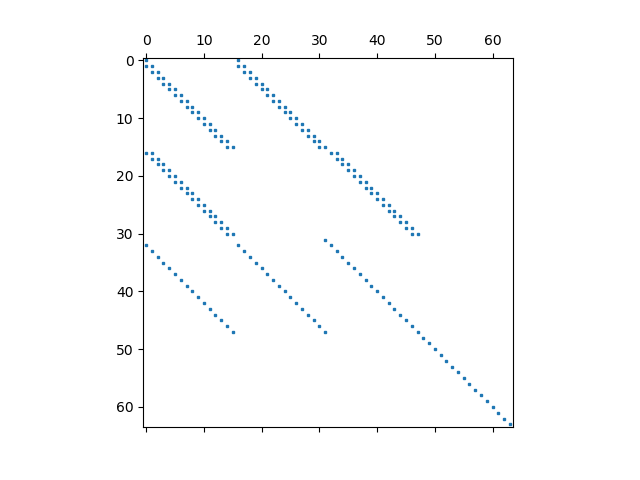
\includegraphics[width=0.60\textwidth]{c16_cpl_sparse.png}
  \end{center}
  \caption{Compressible nozzle with 16 stations, sparsity pattern for coupled matrix.}
  \label{fig-c16-cpl-sparse}
\end{figure}

\Cref{tab-imp-comp} provides details for a range of mesh sizes for
compressible implicit  matrices. The dimensions of the Hermitian matrix are do the symmetrised
matrix needed by HHL. The number of unitaries are derived from the decomposition of
the Hermitian matrix into Pauli strings.
The number of CFD iterations are those required to reduce the residuals and 
corrections to less than $1 \times 10^{-12}$.

\begin{table}[h]
  \centering
  \begin{tabular}{c c c c c c c}
    \toprule
    Nstations & Hermitian matrix &  $\lambda_{min}$ & $\lambda_{max}$ & $\kappa$ & Nunitaries & CFD iterations \\
    \midrule
     8   &   64x64     &$1.9\times10^{-2}$ & 3.01      & 157      & 416   &  96    \\  
     16  &  128x128    &$8.9\times10^{-3}$ & 3.28      & 369      & 1,024 &  177   \\  
     32  &  256x256    &$3.7\times10^{-3}$ & 3.51      & 941      & 2,432 &  410   \\  
     64  &  512x512    &$1.4\times10^{-3}$ & 3.65      & 2,556    & 5,632 &  1,004 \\
    \bottomrule
  \end{tabular}
  \caption{Compressible implicit matrices. 
           Dimensions, eigenvalue range, condition number and unitaries in LCU.
           Sampled after 100 iterations. Pressure ratio = 0.75}
  \label{tab-imp-comp}
\end{table}

From the above derivation, it can be seen that there are additional highly non-linear 
terms in the compressible discretisation, particularly for the effective pressure.
Whilst it is possible to recursively linearise these, it tends to produce an unstable
discretisation. Indeed it is often necessary to apply relaxation to the initial coupled 
iterations and perform some pre-SIMPLE iterations to provide a better initial guess. 
The compressible implicit solver still provides a factor of 3-4 speed-up relative to the 
compressible SIMPLE solver, see \Cref{tab-imp-comp} and \Cref{tab-pc-comp},
but is much less effective than for incompressible flows.



% Incompressible SIMPLE
% ---------------------
\subsubsection{Incompressible SIMPLE solver}
\label{subsubsec-inco-simple}

We follow the discretisation implemented in Appendix D of \cite{gupta1993development}.
First of all we solve the momentum equation \Cref{eqn-euler-1d-disc2} using a Jacobi scheme:

\begin{equation}
  \delta u_i = \frac{R_u^i}{\rho u_{i-\frac{1}{2}}}
  \label{eqn-simple-inco-umom}
\end{equation}

All the $\delta u_i$ terms are evaluated at each station before being used to update
the velocities. This equation is solved on the classical device as the calculation
of $\delta u_i$ can be overlapped with the matrix assembly. Note that the pressures 
are not updated at this stage as they are done separately using the pressure correction 
equation. The SIMPLE algorithm falls into a broader class of {\it segregated} solves.

To solve the continuity equation, the momentum equation is assumed to have been solved,
allowing the velocity and pressure corrections to be related by:

\begin{equation}
  \begin{array}{rcl}
    \delta u_i &=& -\frac{1}{\rho u_{i-\frac{1}{2}}} (\delta p_i - \delta p_{i-1}) \\[8pt]
    \delta u_{i+1} &=& -\frac{1}{\rho u_{i+\frac{1}{2}}} (\delta p_{i+1} - \delta p_{i})
  \end{array}
  \label{eqn-simple-inco-dudp}
\end{equation}

Note that the first equation is based on the momentum equation for station $i$ and
the second equation on the one at for station $i+1$.
These equations can be substituted into the continuity equation \Cref{eqn-euler-1d-disc3}
at station $i$ to give

\begin{equation}
    -\frac{A_{i+1}}{u_{i+\frac{1}{2}}} (\delta p_{i+1} - \delta p_{i})
    +\frac{A_{i}}{u_{i-\frac{1}{2}}} (\delta p_{i} - \delta p_{i-1}) = R_p^i 
  \label{eqn-simple-inco-pceqn1}
\end{equation}

Setting $a_i = \frac{A_{i}}{u_{i-\frac{1}{2}}}$, \Cref{eqn-simple-inco-pceqn1} can
be written as:

\begin{equation}
    -a_{i}\delta p_{i-1} + (a_{i} + a_{i+1})\delta p_{i} - a_{i+1}\delta p_{i+1}
    = R_p^i 
  \label{eqn-simple-inco-pceqn2}
\end{equation}

This leads to a matrix equation of the form $A^p \ket{\delta p} = \ket{R^p}$
which has the sparsity pattern shown \Cref{fig-i16-sim-sparse}.


\begin{figure}[h]
  \begin{center}
    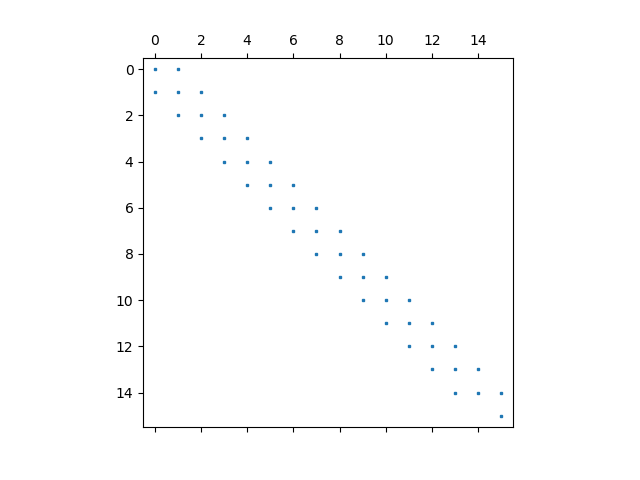
\includegraphics[width=0.60\textwidth]{i16_sim_sparse.png}
  \end{center}
  \caption{Incompressible nozzle with 16 stations, sparsity pattern for pressure correction matrix.}
  \label{fig-i16-sim-sparse}
\end{figure}

Once the pressure correction has been solved, $\ket{\delta p}$ is used to an update to the
velocity field using corrections according to \Cref{eqn-simple-inco-dudp}.
Since the continuity equation is linear for incompressible flows, this results in a 
velocity field that exact satisfies continuity. This step is also completed on the
classical device as it does not require a matrix solution. 

\Cref{tab-pc-incomp} provides details for a range of mesh sizes for 
incompressible pressure corrections matrices. 
The dimensions of the Hermitian matrix are do the symmetrised
matrix needed by HHL. The number of unitaries are derived from the decomposition of
the Hermitian matrix into Pauli strings.
The number of CFD iterations are those required to reduce the residuals and 
corrections to less than $1 \times 10^{-12}$.


\begin{table}[h]
  \centering
  \begin{tabular}{c c c c c c c}
    \toprule
    Nstations & Hermitian matrix &  $\lambda_{min}$ & $\lambda_{max}$ & $\kappa$ & Nunitaries & CFD iterations \\
    \midrule
     8   &   16x16     &$1.4\times10^{-1}$ & 3.18      & 23.3     & 24  & 194   \\
     16  &   32x32     &$3.5\times10^{-2}$ & 3.36      & 97.4     & 56  & 389   \\
     32  &   64x64     &$8.7\times10^{-3}$ & 3.56      & 410      & 128 & 765   \\
     64  &  128x128    &$2.1\times10^{-3}$ & 3.81      & 1,747    & 288 & 1,491 \\
    \bottomrule
  \end{tabular}
  \caption{Incompressible pressure correction matrices.
           dimensions, eigenvalue range, condition number and unitaries in LCU.
           Sampled after after 10 iterations. Area contraction = 10\%.}
  \label{tab-pc-incomp}
\end{table}



% Compressible SIMPLE
% -------------------
\subsubsection{Compressible SIMPLE solver}
\label{subsubsec-comp-simple}

The compressible pressure correction equation follows the derivation of the
incompressible equation except that the additional terms in $\delta \rho$ are 
replaced by $\delta p$ terms using the the gas law. 
We follow \cite{gupta1993development} and used a fully upwinded effective pressure
for the gas law.
This produces a pressure correction matrix with the same sparsity pattern as 
\Cref{fig-i16-sim-sparse}.


\Cref{tab-pc-comp} provides details for a range of mesh sizes for 
compressible pressure corrections matrices. 
The dimensions of the Hermitian matrix are do the symmetrised
matrix needed by HHL. The number of unitaries are derived from the decomposition of
the Hermitian matrix into Pauli strings.
The number of CFD iterations are those required to reduce the residuals and 
corrections to less than $1 \times 10^{-12}$.

\begin{table}[h]
  \centering
  \begin{tabular}{c c c c c c c}
    \toprule
    Nstations & Hermitian matrix &  $\lambda_{min}$ & $\lambda_{max}$ & $\kappa$ & Nunitaries & CFD iterations \\
    \midrule
     8   &   16x16     & $4.8\times10^{-1}$ & 6.89    & 14.3     & 32  & 424   \\
     16  &   32x32     & $1.9\times10^{-1}$ & 8.22    & 42.9     & 80  & 700   \\
     32  &   64x64     & $7.1\times10^{-2}$ & 9.25    & 131      & 192 & 1,449 \\
     64  &  128x128    & $3.0\times10^{-2}$ & 10.1    & 341      & 448 & 2,884 \\
    \bottomrule
  \end{tabular}
  \caption{Compressible pressure correction matrices.
           Dimensions, eigenvalue range, condition number and unitaries in LCU
           for the compressible nozzle.(sampled after 100 iterations).}
  \label{tab-pc-comp}
\end{table}


%
% Core CFD solver
% -------------
\section{Core CFD solver}
\label{sec-corecfd}

The core CFD solver is written in C with a Python wrapper written using ctypes.
The C code is self contained and does not rely on any third party libraries other
than those provided by the compiler. e.g. libm on Linux.


%
% C Build
% -------
\subsection{Building the C code}
\label{subsec-buildc}


\subsubsection{Linux based systems}
The C code can be built as a stand-alone executable or as a library to be linked to a Python code.

\begin{itemize}
\item To make the C executable, type {\tt make} in the {\tt src} directory.
The executable {\tt nozzle} is placed in the {\tt bin} directory.

\item To make the C library, type {\tt make lib} in the {\tt src} directory.
The shared object library {\tt libnozzle.so} is placed in the {\tt lib} directory.

\item To rebuild from scratch , type  {\tt make clean} in the {\tt src} directory.
\end{itemize}


\subsubsection{Windows based systems}

Not cuurently supported.



%
% Running the code
% ----------------
\subsection{Running the code}
\label{subsec-run}

There are 3 modes of running the code include in the distribution.

\begin{itemize}
\item To run the C-code directly type: {\tt [path]/bin/nozzle -i [path]inputfile.xml}.

      Typing {\tt [path]/bin/nozzle -h} gives a short list of the input options.

      Sample input files are included in the {\tt input} directory of the distribution.
      Note each input file can be run in the four possible combinations of incompressible/compressible flow and
      SIMPLE/coupled solvers. Which combination is run is determined by the {\tt setup} section of the
      input file as described in \Cref{subsec-ifile}.

\item To run the C solver as a library call from Python type: {\tt [path]/script/run\_cprog.py -i [path]inputfile.xml}.

      This simply demonstrates the infrastructure used to call the C library from within a Python script.

\item To use the C library to set-up matrices to be solved using the {\tt scipy} linear algebra routine type:
      {\tt [path]/script/run\_pysolve.py -i [path]inputfile.xml}.  
\end{itemize}

The final option provides a template for replacing the {\tt scipy} linear solver with a quantum linear equation solver
as described in \Cref{subsec-qles}.


%
% Python C interface
% ------------------
\subsection{Python-C interface}
\label{subsec-py2c}
There are two layers to the Python-C interface:
\begin{itemize}
  \item Data instantiation when python is the main routine.
  \item Data exchange to {\it get} a matrix and a right-hand side vector, 
        and to {\it put} a solution vector.
\end{itemize}

Both of these depend on sharing C structures with the Python code.


%
% Data instantiation
% ------------------
\subsubsection{Data instantiation}
\label{subsubsec-data-inst}

\Cref{list-noz-cstruct} shows the high level structure used by the C solver.
As can be seen, this is a structure of structures which, collectively, contain all the
data used by the solver. These are not further defined here as they are not needed by
the Python layer.

\begin{lstlisting}[numbers=left, language=C, caption=C master structure for nozzle data, label=list-noz-cstruct]
typedef struct
{
        SETUP   *setup;
        MESH    *mesh;
        FLOW    *flow;
        SOLVER  *solver;
        FILES   *files;
        ARRAYS  *arrays;
        HISTORY *history;
} NOZZLE;
\end{lstlisting}

In fact, the Python layer needs only manage the pointer which it can do by treating it
as a {\tt void}. The only data passed between the C and Python layers is the memory address of
the nozzle pointer.
\Cref{list-noz-pyinst} gives code segments which call C routines to instantiate an empty nozzle structure;
load data from an input file; and, free the structure after the calculations have been completed.
Note that the call to {\tt c\_lib.c2py\_noz\_create} on line 2 passes the pointer by reference. 
This is needed because the memory for the pointer is allocated with the C code, so it must return
a pointer to a pointer.
The variable {\tt i\_cptr} on line 4 is the name of the input file that is read as a command 
line option.


\begin{lstlisting}[numbers=left, language=Python, caption=Python instantiation., label=list-noz-pyinst]
    noz_cptr = c_void_p()
    c_lib.c2py_noz_create(byref(noz_cptr))
    ...
    c_lib.c2py_read_input(i_cptr, noz_cptr)
    ...
    c_lib.c2py_noz_free(noz_cptr)
\end{lstlisting}

%
% Data exchange
% -------------
\subsubsection{Data exchange}
\label{subsubsec-data-exch}

In order to investigate quantum linear solvers, it is necessary to share matrices and vectors
between the C and Python layers. This is done by using a common structure definition.
\Cref{list-smat-cstruct} shows the C structure and \Cref{list-smat-pystruct} shows the
corresponding Python structure. Both used the same compressed row format.

\begin{lstlisting}[numbers=left, language=C, caption=C sparse matrix structure., label=list-smat-cstruct]
typedef struct
{
        int32_t nr;
        int32_t nc;
        int32_t nnz;
        int32_t *col;
        int32_t *rst;
        double  *val;
        double  *b;
} SMATRIX;
\end{lstlisting}

Note that integers are declared as {\tt int32} to ensure both the C and Python layers use 
32 bit integers.
Note that the sparse matrix structures also includes the residual, or right hand side vector, {\tt b}.
This is a convenience as both the matrix and vector can be retrieved in a single call.
It is also convenient on the C side as the matrix entries and residuals are computed at the
same time.
The solution vector is computed separately and, therefore, not included in the structure.


\begin{lstlisting}[numbers=left, language=Python, caption=Python sparse matrix structure., label=list-smat-pystruct]
class SMATRIX(Structure):
      _fields_ = [("nr",  c_int32),
                  ("nc",  c_int32),
                  ("nnz", c_int32),
                  ("col", POINTER(c_int32)),
                  ("rst", POINTER(c_int32)),
                  ("val", POINTER(c_double)),
                  ("b",   POINTER(c_double))
                 ]
      _defaults_ = {"nr" : 0,
                    "nc" : 0,
                    "nnz": 0,
                    "col": None,
                    "rst": None,
                    "val": None,
                    "b"  : None}
\end{lstlisting}


\Cref{list-get-smat} shows how to {\it get} a matrix and vector from the C code and
convert them to a scipy sparse matrix and numpy vector.
This is taken from the script {\tt run\_pysolve.py}
On line 10, the {\tt scipy.sparse.linalg} spsolve routine is used to solve for {\tt x}.
Lines 12-13 show how to {\it put} the solution vector back into the C code.


\begin{lstlisting}[numbers=left, language=Python, caption=Code segment for Python-C matrix and vector exchange., label=list-get-smat]
    S = SMATRIX()
    c_lib.c2py_get_smat(noz_cptr, byref(S))

    col = np.ctypeslib.as_array(S.col, shape=(S.nnz,))
    rst = np.ctypeslib.as_array(S.rst, shape=(S.nr+1,))
    val = np.ctypeslib.as_array(S.val, shape=(S.nnz,))
    b   = np.ctypeslib.as_array(S.b,   shape=(S.nr,))

    SP = sparse.csr_matrix((val, col, rst),shape=(S.nr, S.nc), dtype=np.double)
    x  = spsolve(SP, b)

    xc = x.ctypes.data_as(POINTER(c_double))
    rc = c_lib.c2py_put_soln(noz_cptr, xc)
\end{lstlisting}

As can be seen, the above code segments are independent of the CFD flow type and solution scheme.
These are contained within the C layer and controlled via a single input file.



%
% QLES solver
% ----------
\subsection{Linking to a quantum linear equation solver}
\label{subsec-qles}

In principle, linking to a quantum solver is {\it just} a matter of replacing the call to
{\tt spsolve} in line 10 of \Cref{list-get-smat} with a call to the equivalent quantum solver.
However, the quantum solver is likely to need a lot of additional input, including additional
data such as phase factors for QSVT.
The user has a choice to hardwire them for initial development testing, add them as additonal 
input options to the python script, or include them in an auxillary input file.

Note that the call to {\tt spsolve} is within an iterative loop. Only data that changes as part of the
non-linear outer iterations should be included within the loop.
Data input and set-up should be outside the loop.

It is recommended to make a copy of the file {\tt run\_pysolve.py} and use that as a template 
for the QLES solver.


%
% Input file
% ----------
\subsection{Input file}
\label{subsec-ifile}

There are sample input files in the {\tt input} directory of the distribution.
The files are structured to include options for all combinations of flow type and solver.
The choice to be run is controlled by the {\tt setup} section as described in \Cref{subsubsec-ifile-overview}.
If files need to be simplified, the sections for the unused options can be removed. 

%
% overview
% --------
\subsubsection{Overview}
\label{subsubsec-ifile-overview}

The input file has been designed for all 4 combinations of flow regime and
solver type to be held in a single file with two binary flags to select which option is executed.
This adds some verbosity to the file but eases the number of files that need to be managed.
This does not prevent separate files being used for separate cases if that is preferred.
The high-level structure of the file is shown in  \Cref{list-xml01}.

\begin{lstlisting}[numbers=left, language=xml, caption=Input file main sections., label=list-xml01]
<?xml version="1.0" encoding="UTF-8"?>
<nozzle>
  <setup>
    <casename>nozzle</casename>
    <compressible>0</compressible>
    <couple>1</couple>
  </setup>

  <mesh>...</mesh>

  <incompressible>
    <flow>...</flow>
    <solver>
      <simple>...</simple>
      <couple>...</couple>
    </solver>
  </incompressible>

  <compressible>
    <flow>...</flow>
    <solver>
      <simple>...</simple>
      <couple>...</couple>
    </solver>
  </compressible>
</nozzle>
\end{lstlisting}


The {\tt setup} section contains a case name and binary variables to
toggle the flow and solver types. 
This section in \Cref{list-xml01} specifies incompressible flow using the coupled solver.
See \Cref{subsubsec-naming} for how the case name is used to set the names of the 
output files based on the setup.

The {\tt mesh} section is common to all setup combinations and is described below.
There are separate sections for incompressible and compressible flow with
each containing {\tt flow} and {\tt solver} sections.
The solver sections contain separate {\tt simple} and {\tt couple} sections for
each solver type. As shown below, the variables in each section depend on the
set-up and where variables have the same name they generally have different values,
according to the section they are in. 

All variables have default values. Those variables that use the default values can
be omitted from the input file for brevity, if desired.


%
% mesh
% ----
\subsubsection{Mesh data}

\Cref{list-xml02} shows the {\tt mesh} section of the input file.

\begin{lstlisting}[numbers=left, language=xml, caption=Input file mesh section., label=list-xml02]
  <mesh>
    <nx>16</nx>
    <ain>1.0</ain>
    <da>-0.1</da>
  </mesh>
\end{lstlisting}

The variables are:
\begin{itemize}
  \item{\tt nx} -  the number of axial stations in the mesh, this value is used as part
                   of the output file names.
  \item{\tt ain} - for incompressible flows this is the inlet area of the channel.
                   For compressible flows this is a scale factor for the inlet area,
                   which  can be used to scale the matrix entries but is usually set to {\tt 1.0}.
  \item{\tt da}  - the area contraction at the midpoint of the channel for incompressible flows.
                   This is specified as a fraction of the inlet area and is negative for an
                   area contraction and positive for an area expansion.
\end{itemize}


%
% incomp-simple
% -------------
\subsubsection{Incompressible flow, SIMPLE solver}
\label{subsubsec-insi-xml}

\Cref{list-xml03} shows the section of the input file for incompressible flow with the SIMPLE solver.
Note that all flow variables are non-dimensional.

\begin{lstlisting}[numbers=left, language=xml, caption=Input file for incompressible + SIMPLE solver., label=list-xml03]
  <incompressible>
    <flow>
      <rho>1.0</rho>                   <!-- constant density -->
      <bc>
        <ptin>1.5</ptin>               <!-- inlet total pressure -->
        <pex>0.95</pex>                <!-- exit static pressure -->
      </bc>
    </flow>

    <solver>
      <simple>
        <niters>2000</niters>          <!-- number of iterations -->
        <relaxu>1.0</relaxu>           <!-- u-relaxation factor -->
        <relaxp>1.0</relaxp>           <!-- p-relaxation factor -->
        <toleru>1.0e-12</toleru>       <!-- u-convergence tolerance -->
        <tolerp>1.0e-12</tolerp>       <!-- p-convergence tolerance -->
      </simple>
    </solver>
  </incompressible>
\end{lstlisting}

The variables are defined in \Cref{list-xml03} and should be self-explanatory.
As shown in \Cref{tab-pc-incomp}, the number of iterations varies considerably
for different mesh sizes. 
{\tt niters} is the maximum number of iterations, the calculation will terminate
when it reaches either {\tt niters} or both of the convergence tolerances have been meet.


%
% incomp-couple
% -------------
\subsubsection{Incompressible flow, coupled solver}
\label{subsubsec-inco-xml}

\Cref{list-xml04} shows the section of the input file for incompressible flow with the coupled solver.
Note that all flow variables are non-dimensional.

\begin{lstlisting}[numbers=left, language=xml, caption=Input file for incompressible + coupled solver., label=list-xml04]
  <incompressible>
    <flow>...  </flow>

    <solver>
      <couple>
        <niters>10</niters>            <!-- number of iterations -->
        <presim>0</presim>             <!-- number SIMPLE iterations before coupled solver -->
        <relaxc>1.0</relaxc>           <!-- relaxation factor applied to all variables -->
        <rrampc>0</rrampc>             <!-- number of iterations over which to ramp relaxc -->
        <tolerc>1.0e-12</tolerc>       <!-- convergence tolerance for all variables -->
      </couple>
    </solver>
  </incompressible>
\end{lstlisting}

The {\tt flow} is not included as it is identical to \Cref{list-xml03}.
The number of iterations is as before, but has a much smaller value as \Cref{tab-imp-comp}
shows that number of iterations is less than 10 for all mesh sizes.
A single convergence tolerance, {\tt tolerc}, is used for the coupled set of equations.
The variables {\tt presim}, {\tt relaxc} and {\tt rrampc} are needed for the compressible 
coupled solver and are described in \Cref{subsubsec-coco-xml}. 
The values of these variables in \Cref{list-xml04} are the defaults and these can be omitted
from the input file for incompressible flows.


%
% comp-simple
% -------------
\subsubsection{Compressible flow, SIMPLE solver}
\label{subsubsec-cosi-xml}

\Cref{list-xml05} shows the section of the input file for compressible flow with the SIMPLE solver.
Note that all flow variables are non-dimensional.

\begin{lstlisting}[numbers=left, language=xml, caption=Input file for incompressible + SIMPLE solver., label=list-xml05]
  <compressible>
    <flow>
      <bc>
        <ptin>1.5</ptin>               <!-- inlet total pressure -->
        <min>0.8</min>                 <!-- inlet Mach number -->
        <pex>0.75</pex>                <!-- exit static pressure -->
      </bc>
      <gaslaw>
        <gamma>1.4</gamma>             <!-- ratio of specific heats -->
        <cp>3.5</cp>                   <!-- specific heat at constant pressure -->
        <rgas>1.0</rgas>               <!-- perfect gas constant -->
        <upwind>2</upwind>             <!-- 1, 2,3 for 1st, 2nd and 3-pt density upwinding -->
      </gaslaw>
    </flow>

    <solver>
      <simple>
        <niters>5000</niters>          <!-- number of iterations -->
        <relaxu>1.0</relaxu>           <!-- u-relaxation factor -->
        <relaxp>1.0</relaxp>           <!-- p-relaxation factor -->
        <toleru>1.0e-12</toleru>       <!-- u-convergence tolerance -->
        <tolerp>1.0e-12</tolerp>       <!-- p-convergence tolerance -->
      </simple>
    </solver>
  </compressible>
\end{lstlisting}

%
% comp-couple
% -------------
\subsubsection{Compressible flow, coupled solver}
\label{subsubsec-coco-xml}

\Cref{list-xml06} shows the section of the input file for compressible flow with the coupled solver.
Note that all flow variables are non-dimensional.

\begin{lstlisting}[numbers=left, language=xml, caption=Input file for incompressible + coupled solver., label=list-xml06]
  <compressible>
    <flow>...</flow>

    <solver>
      <couple>
        <niters>2000</niters>          <!-- number of iterations -->
        <presim>10</presim>            <!-- number SIMPLE iterations before coupled solver -->
        <relaxc>0.75</relaxc>          <!-- relaxation factor applied to all variables -->
        <rrampc>20</rrampc>            <!-- number of iterations over which to ramp relaxc -->
        <tolerc>1.0e-12</tolerc>       <!-- convergence tolerance for all variables -->
      </couple>
    </solver>
  </compressible>
\end{lstlisting}





%
% Output file
% -----------
\subsection{Output files}
\label{subsec-ofile}

\subsubsection{File naming convention}
\label{subsubsec-naming}

There are two output files: a convergence history and a flow solution file. 
The naming convention for both files is \textit{casename\_nx\_ffss.ext}, where:
\begin{itemize}
\item \textit{casename} is the user specified name in the input file.
\item \textit{nx} is the number of stations.
\item \textit{ff} is a two character identifier for the flow type: \textit{in} for
      incompressible flow or \textit{co} for compressible flow.
\item \textit{ss} is a two character identifier for the solver type: \textit{si} for
      the SIMPLE solver or \textit{co} for the coupled solver.
\item \textit{ext} is the three character file extension: \textit{hst} for the convergence
      history file and \textit{sol} for the solution file.
\end{itemize}

For example, the history file for an incompressible SIMPLE case named 'nozzle with 16 stations is
{\tt nozzle\_016\_insi.hst}.
If cases with more that 999 stations are needed, modify the routine {\tt noz\_files} to change the
format statement in the {\tt snprintf} statements to increase '3' to the number of digits needed.



\subsubsection{Convergence history}
\label{subsubsec-form-conv}

The contents of the convergence history file depend on the flow type.
In both cases the file contains the root mean square (RMS) of the changes in the flow variables between
the current iteration and the previous one; and, the residual errors, e.g $R^u$, of the flow equations
at the start of the iteration.
Both should reduce towards the convergence tolerance as the iterations proceed.
For incompressible cases, the history file contains the RMS changes for $u$ and $p$ and the RMS resisuals
of the momentum and continuity equations.
For compressible flows, the RMS changes in density and residual of the gas equation are also included.
Sample files for both flow types are listed below, showing the first 9 iterations.

See \Cref{subsec-res-conv} for details on how to plot the convergence history of a single run and
to compare the convergence histories of multiple runs.

\begin{verbatim}
head nozzle_016_insi.hst
"iter",  "du_rms",        "dp_rms",        "resu_rms",      "resp_rms"
 1,  0.00000000e+00,  9.95624279e-02,  0.00000000e+00,  1.62406810e-02
 2,  3.42680753e-02,  9.21423809e-02,  3.56263102e-02,  2.32527299e-02
 3,  4.09420463e-03,  1.56536726e-03,  4.31829249e-03,  1.56084554e-03
 4,  3.82501330e-03,  2.49477798e-03,  4.06783477e-03,  8.77342756e-04
 5,  3.60318337e-03,  2.36292698e-03,  3.84504091e-03,  8.24039930e-04
 6,  3.39492043e-03,  2.23327519e-03,  3.63437959e-03,  7.76310997e-04
 7,  3.19933160e-03,  2.11074512e-03,  3.43527772e-03,  7.31505443e-04
 8,  3.01557136e-03,  1.99495898e-03,  3.24709921e-03,  6.89419128e-04
 9,  2.84285931e-03,  1.88554307e-03,  3.06924290e-03,  6.49871476e-04


head nozzle_016_coco.hst
"iter", "du_rms",    "dp_rms",     "dr_rms",    "resu_rms",   "resp_rms",   "resr_rms"
 1,  2.29801e-01,  5.03378e-02,  2.88455e-02,  1.07241e-02,  2.03448e-02,  2.03448e-02
 2,  2.58647e-01,  1.51207e-01,  1.17747e-01,  5.94100e-03,  5.40709e-03,  5.40709e-03
 3,  8.72627e-01,  5.95568e-01,  4.75178e-01,  4.18458e-03,  6.25604e-03,  6.25604e-03
 4,  3.39289e-01,  2.75104e-01,  2.11024e-01,  1.35157e-01,  2.57616e-01,  2.57616e-01
 5,  1.13501e+00,  5.81302e-01,  3.79980e-01,  1.81180e-01,  5.31819e-02,  5.31819e-02
 6,  4.67940e-01,  2.83047e-01,  2.98249e-01,  1.93246e-01,  3.24966e-01,  3.24966e-01
 7,  2.68325e-01,  1.12835e-01,  9.90863e-02,  5.66960e-02,  1.91540e-01,  1.91540e-01
 8,  2.00619e-01,  1.24138e-01,  7.90677e-02,  2.57842e-02,  6.30679e-02,  6.30679e-02
 9,  3.47459e-01,  2.28170e-01,  1.64274e-01,  8.91253e-03,  1.89085e-02,  1.89085e-02
\end{verbatim}

Note that the precision of the compressible file has been truncated for the purposes of 
illustrating the file format. The actual file has the same precision as the incompressible file.


\subsubsection{Flow field}
\label{subsubsec-form-flow}

As with the convergence histories, the format of the solution files depends on whether
incompressible or compressible flow has been modelled.
Sample files for both flow types are listed below, showing the solution with 8 axial
stations.

See \Cref{subsec-res-flow} for details on how to plot the flow field of a single run and
to compare the flow fields of multiple runs.


\begin{verbatim}
head nozzle_008_insi.sol 
"index", "x",        "area",    "density",  "velocity",  "pressure"
 1,  0.00000000,  1.00000000,  1.00000000,  0.99352315,  1.00645586
 2,  0.14285714,  0.95002040,  1.00000000,  1.05396039,  0.93273107
 3,  0.28571428,  0.91778253,  1.00000000,  1.09468920,  0.87557899
 4,  0.42857142,  0.90196380,  1.00000000,  1.12077187,  0.83702077
 5,  0.57142857,  0.90196380,  1.00000000,  1.12039273,  0.83109312
 6,  0.71428571,  0.91778253,  1.00000000,  1.10510955,  0.84489365
 7,  0.85714285,  0.95002040,  1.00000000,  1.06576098,  0.88937807
 8,  1.00000000,  1.00000000,  1.00000000,  1.01185327,  0.95000000


head nozzle_008_cosi.sol 
"index", "x",     "area", "density","velocity","pressure",    "temp",  "Mach no"
 1,  0.000000,  1.038230,  0.733619,  0.903193,  0.648126,  0.883463,  0.812124
 2,  0.142857,  1.002814,  0.673123,  1.019130,  0.569949,  0.851624,  0.933340
 3,  0.285714,  1.005860,  0.594401,  1.150608,  0.479892,  0.810871,  1.079907
 4,  0.428571,  1.039360,  0.524993,  1.260737,  0.405785,  0.772934,  1.211963
 5,  0.571428,  1.099747,  0.448136,  1.395860,  0.318806,  0.721653,  1.388716
 6,  0.714285,  1.185954,  0.441964,  1.312472,  0.369072,  0.753916,  1.277511
 7,  0.857142,  1.298492,  0.629288,  0.841891,  0.630211,  0.898745,  0.750540
 8,  1.000000,  1.438982,  0.791263,  0.604183,  0.750000,  0.947851,  0.524487

\end{verbatim}

As before, the precision of the output has been truncated for the purposes of illustrating 
the file format.



%
% Results
% -------
\section{Analysing the results}
\label{sec-results}


%
% Convergence
% -----------
\subsection{Convergence histories}
\label{subsec-res-conv}

Up to 5 convergence history files can be compared using the script
{tt plot\_hist.py}. 
As described in \Cref{subsubsec-form-conv} the format of the plot depends on
the type of flow.

\Cref{fig-plot-hst-coco} illustrates how to compare the convergence of the
coupled compressible solver on three different meshes using the following command:

\begin{verbatim}
./plot_hist.py nozzle_008_coco.hst nozzle_016_coco.hst nozzle_032_coco.hst
\end{verbatim}

The file names are used as the legends for each line in the plot.

\begin{figure}[ht]
  \begin{center}
    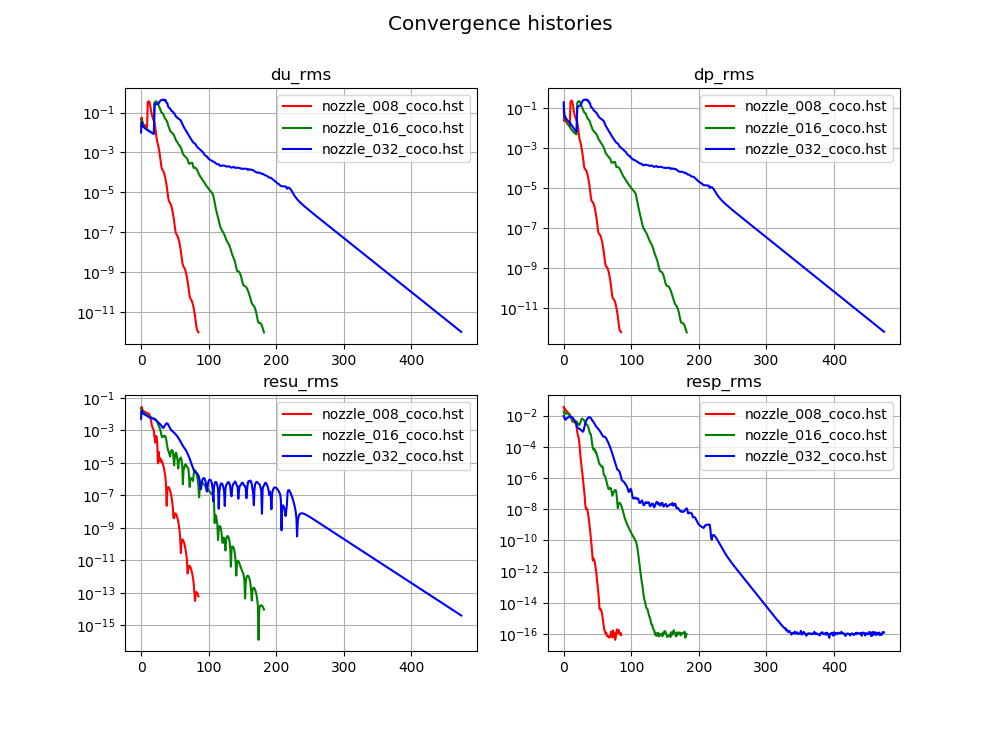
\includegraphics[width=0.70\textwidth]{plot-hst-coco.png}
  \end{center}
  \caption{Convergence history plot for the coupled compressible solver on three different meshes.}
  \label{fig-plot-hst-coco}
\end{figure}



%
% Flow field
% ----------
\subsection{Flow field}
\label{subsec-res-flow}

Up to 5 flow solution files can be compared using the script
{tt plot\_sol.py}. 
As described in \Cref{subsubsec-form-flow} the format of the plot depends on
the type of flow.

\Cref{fig-plot-sol-coco} illustrates how to compare the solutions of the
coupled compressible solver on three different meshes using the following command:

\begin{verbatim}
./plot_sol.py nozzle_008_coco.sol nozzle_016_coco.sol nozzle_032_coco.sol
\end{verbatim}

The plots illustrate how the shock wave becomes sharper as the resolution of the mesh increases.

\begin{figure}[ht]
  \begin{center}
    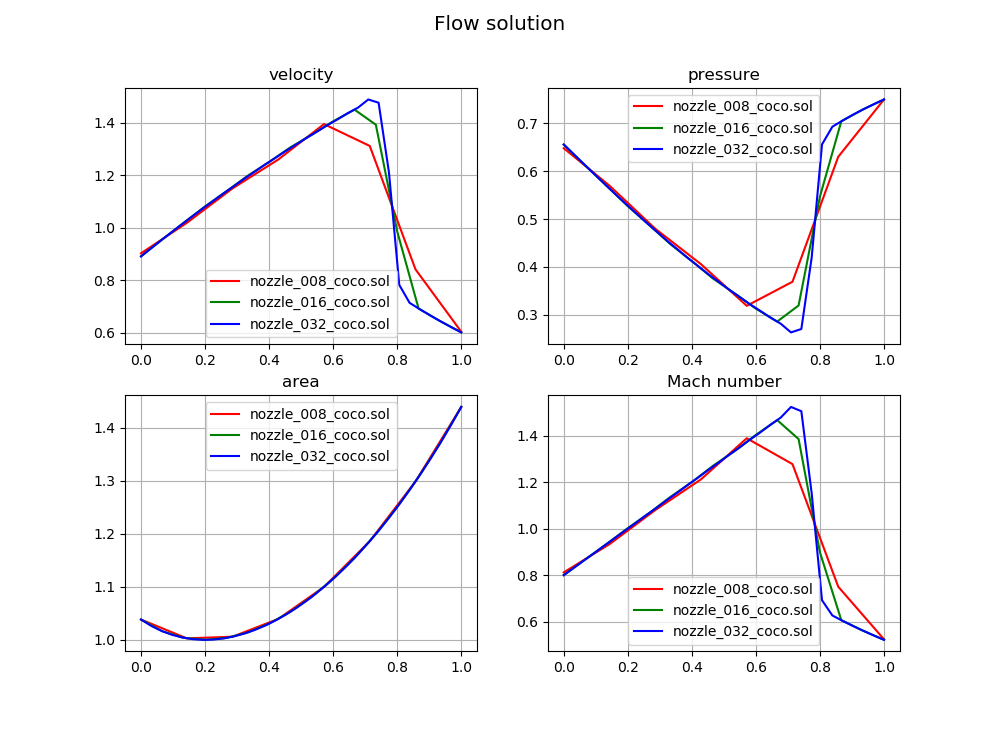
\includegraphics[width=0.70\textwidth]{plot-sol-coco.png}
  \end{center}
  \caption{Flow solution plot for the coupled compressible solver on three different meshes.}
  \label{fig-plot-sol-coco}
\end{figure}


\Cref{fig-plot-sol-inco} illustrates how to compare the solutions of the
coupled incompressible solver on three different meshes using the following command:

\begin{verbatim}
./plot_sol.py nozzle_008_inco.sol nozzle_016_inco.sol nozzle_032_inco.sol
\end{verbatim}

This illustrates different nature of the incompressible where the flow is symmetric about the 
centre of the nozzle.

\begin{figure}[ht]
  \begin{center}
    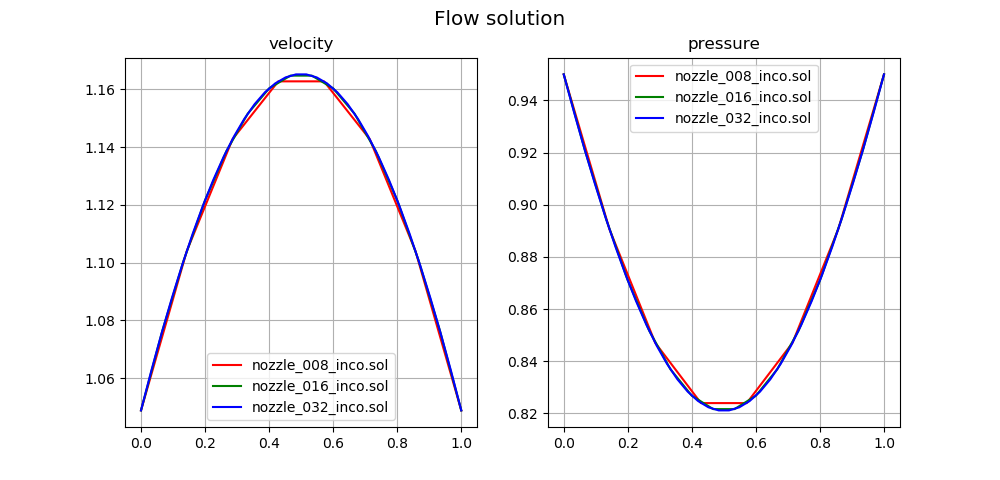
\includegraphics[width=0.70\textwidth]{plot-sol-inco.png}
  \end{center}
  \caption{Flow solution plot for the coupled incompressible solver on three different meshes.}
  \label{fig-plot-sol-inco}
\end{figure}




%
% Summary
% -------
\section{Summary}
\label{sec-summary}

The 1D nozzle solver provides a flexible Python interface for testing quantum linear equation
solvers on fluid flow type problems.
The core CFD solver, written in C, is linked via a library to enable developers to focus on their
quantum solver.
The benefit of the nozzle system is that it allows researchers to investigate the feedback between the 
inner linear system, solved using a quantum algorithm, and the outer classical non-linear update.

Although the solver is only 1 dimensional, there are a range of solver options that can be
used to generate matrices with up to 8 diagonals using the coupled compressible solver. The standard
pressure correction solver has 3 diagonals. The coupled incompressible solver has 6 diagonals and
gives rapid convergence which is useful when emulating the quantum circuit is time-consuming.

The plotting routines enable easy comparison of classical and quantum results.


% References
% ----------
%\addcontentsline{toc}{section}{Bibliography}
\bibliographystyle{plain}
\bibliography{include/references}

\end{document}

